\chapter{Progettazione e codifica}
\label{cap:progettazione-codifica}

%Mettere i mockup di figma con spiegazione
%riportare una analisi del codice e la fatica fatta con firebase


%\intro{Breve introduzione al capitolo}\\

\section{Progettazione}
\label{sec:progettazione}
%partire dicendo di aver progettato l'interfaccia con figma, riportando degli screen dal mio lavoro

Dopo una prima parte di stage dove ho studiato le tecnologie riportare al \hyperref[sec:tecnologie]{terzo capitolo}, ho pensato come sviluppare l'applicazione richiesta.\newline
Di prassi in RiskAPP si utilizza Figma per poter avere una idea più chiara del lavoro che si desidera fare, quindi per prima cosa ho progettato la grafica e la struttura dell'app con l'aiuto di questo software di progettazione.\newline

\begin{figure}[!h] 
    \centering 
    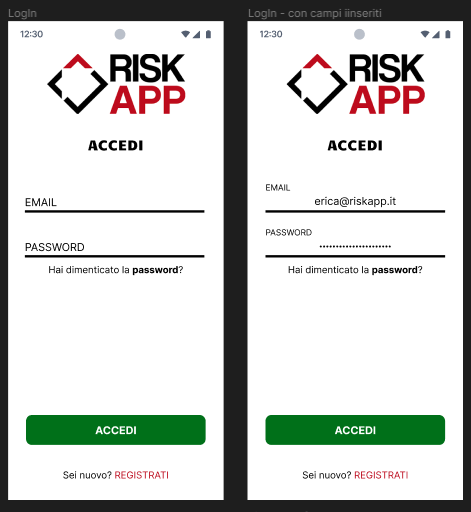
\includegraphics[width=0.9\columnwidth]{figma/accedi} 
    \caption{Schermata Accedi progettata in Figma}
\end{figure}

\begin{figure}[!h] 
    \centering 
    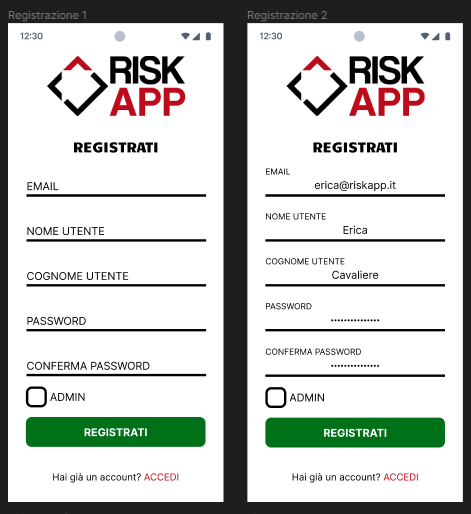
\includegraphics[width=0.9\columnwidth]{figma/registrati} 
    \caption{Schermata Registrati progettata in Figma}
\end{figure}

\begin{figure}[!h] 
    \centering 
    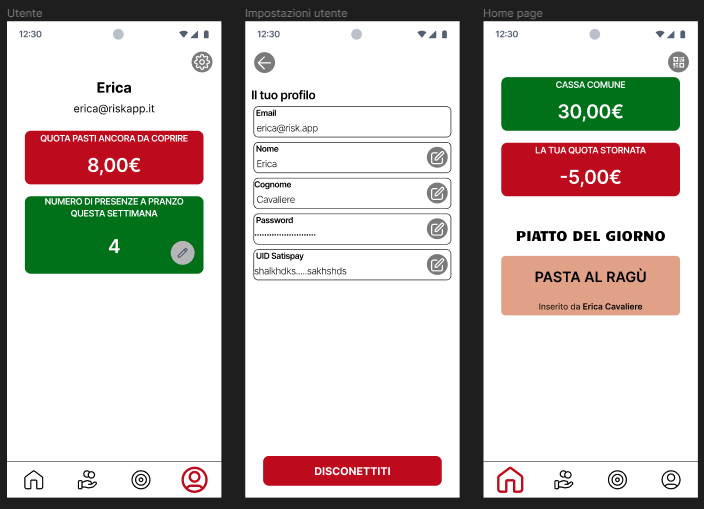
\includegraphics[width=0.9\columnwidth]{figma/esempi} 
    \caption{Alvune schermate progettate in Figma}
\end{figure}

\begin{figure}[!h] 
    \centering 
    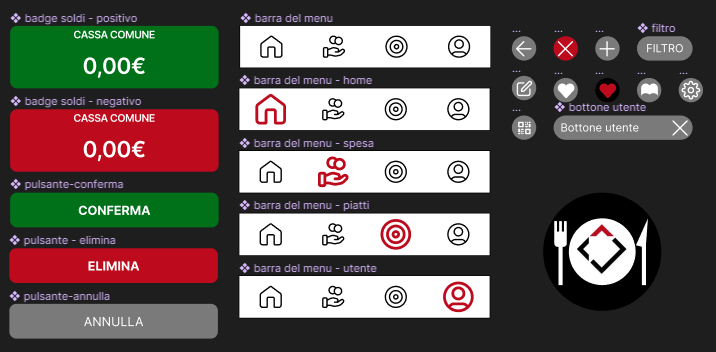
\includegraphics[width=0.9\columnwidth]{figma/container} 
    \caption{Alcuni pulsati e icone progettate in Figma}
\end{figure}

%\subsubsection{Namespace 1} %**************************
%Descrizione namespace 1.
%
%\begin{namespacedesc}
%    \classdesc{Classe 1}{Descrizione classe 1}
%    \classdesc{Classe 2}{Descrizione classe 2}
%\end{namespacedesc}


\section{Design Pattern utilizzati}
%forse parlare dell'MVVM o BLoC patttern

\section{Codifica} %riportare qui il database?
%In questa sezione riporto la struttura della cartella lib, parlerò delle componenti e, del file firebase_option e delle classi
%riportare anche le immagine dell'app creata